\documentclass{article}

% Packages for formatting
\usepackage[margin=1in]{geometry}
\usepackage{fancyhdr}
\usepackage{enumitem}
\usepackage{graphicx}
\usepackage{kotex}
\usepackage{amsmath}
\usepackage{amsthm}
\usepackage{algorithm2e,setspace}
\usepackage{algpseudocode}
\usepackage{xcolor}
\usepackage{amssymb}

% Fonts
\usepackage[T1]{fontenc}
\usepackage[utf8]{inputenc}
\usepackage{newpxtext,newpxmath}
\usepackage{sectsty}

% Define colors
\definecolor{blue1}{HTML}{0077c2}
\definecolor{blue2}{HTML}{00a5e6}
\definecolor{blue3}{HTML}{b3e0ff}
\definecolor{blue4}{HTML}{00293c}
\definecolor{blue5}{HTML}{e6f7ff}

\definecolor{thmcolor}{RGB}{231, 76, 60}
\definecolor{defcolor}{RGB}{52, 152, 219}
\definecolor{lemcolor}{RGB}{155, 89, 182}
\definecolor{corcolor}{RGB}{46, 204, 113}
\definecolor{procolor}{RGB}{241, 196, 15}

\usepackage{color,soul}
\usepackage{soul}
\newcommand{\mathcolorbox}[2]{\colorbox{#1}{$\displaystyle #2$}}
\usepackage{cancel}
\newcommand\crossout[3][black]{\renewcommand\CancelColor{\color{#1}}\cancelto{#2}{#3}}
\newcommand\ncrossout[2][black]{\renewcommand\CancelColor{\color{#1}}\cancel{#2}}

\usepackage{hyperref}
\usepackage{booktabs}

% Chapter formatting
\definecolor{titleblue}{RGB}{0,53,128}
\usepackage{titlesec}
\titleformat{\section}
{\normalfont\sffamily\Large\bfseries\color{titleblue!100!gray}}{\thesection}{1em}{}
\titleformat{\subsection}
{\normalfont\sffamily\large\bfseries\color{titleblue!50!gray}}{\thesubsection}{1em}{}

%Tcolorbox
\usepackage[most]{tcolorbox}

%Tikzpicture
\usepackage{tikz-cd}
\usetikzlibrary{positioning}
\usetikzlibrary{angles, quotes}

% Header and footer formatting
\pagestyle{fancy}
\fancyhead{}
\fancyhf{}
\rhead{Student ID: 20192250\quad Name: 지용현}%\rule{3cm}{0.4pt}}
\lhead{\textcolor{blue2}{\textbf{CA Assignment \#2}}}
% Define footer
\newcommand{\footer}[1]{
	\begin{flushright}
		\vspace{2em}
		
\includegraphics[width=2cm]{school_logo.jpg} \\
		\vspace{1em}
		\textcolor{blue2}{\small\textbf{#1}}
	\end{flushright}
}
%\rfoot{\large Department of Information Security, Cryptogrphy and Mathematics, Kookmin Uni.
\includegraphics[height=1.5cm]{school_logo.jpg}}
\fancyfoot{}
\fancyfoot[C]{-\thepage-}

\newcommand{\ie}{\textnormal{i.e.}}
\newcommand{\rsa}{\mathsf{RSA}}
\newcommand{\rsacrt}{\mathsf{RSA}\textendash\mathsf{CRT}}
\newcommand{\inv}[1]{#1^{-1}}

\usepackage{amsthm}
\newtheorem{axiom}{Axiom}[section]
\newtheorem{theorem}{Theorem}
\newtheorem*{theorem*}{Theorem}
\newtheorem{proposition}[theorem]{Proposition}
\newtheorem{corollary}{Corollary}[theorem]
\newtheorem*{corollary*}{Corollary}
\newtheorem{lemma}[theorem]{Lemma}
\newtheorem*{lemma*}{Lemma}

\theoremstyle{definition}
\newtheorem{definition}{Definition}
\newtheorem*{definition*}{Definition}
\newtheorem{remark}{Remark}
\newtheorem{exercise}{Exercise}[section]

%New Command
\newcommand{\set}[1]{\left\{#1\right\}}
\newcommand{\N}{\mathbb{N}}
\newcommand{\Z}{\mathbb{Z}}
\newcommand{\Q}{\mathbb{Q}}
\newcommand{\R}{\mathbb{R}}
\newcommand{\C}{\mathbb{C}}
\newcommand{\F}{\mathbb{F}}
\newcommand{\nbhd}{\mathcal{N}}
\newcommand{\Log}{\operatorname{Log}}
\newcommand{\Arg}{\operatorname{Arg}}
\newcommand{\pv}{\operatorname{P.V.}}

\newcommand{\of}[1]{\left( #1 \right)} 
\newcommand{\abs}[1]{\left\lvert #1 \right\rvert}
\newcommand{\norm}[1]{\left\| #1 \right\|}

\newcommand{\sol}{\textcolor{magenta}{\bf Sol}}
\newcommand{\conjugate}[1]{\overline{#1}}


\renewcommand{\Re}{\operatorname{Re}}
\renewcommand{\Im}{\operatorname{Im}}

\begin{document}
	\pagenumbering{arabic}
	\begin{center}
		\huge\textbf{Complex Analysis}\\
		\vspace{0.5em}
	\end{center}
	
	\begin{enumerate}
		\item We define \[
		f'\of{t}=\frac{d}{dt}\left[u\of{t}+iv\of{t}\right] = u'\of{t}+iv'\of{t},\quad
		\int f\of{t}dt = \int u\of{t}dt + i\int v\of{t}dt.
		\] \begin{itemize}
			\item[(a)]
			\item[(b)]
			\item[(c)]
		\end{itemize}
		\begin{proof}[\sol]
			\begin{itemize}
				\item[(a)] Note that \[
				f\of{t}=e^{z_0t}=e^{\of{a+ib}t}=e^{at}e^{i bt}=e^{at}\of{\cos\of{bt}+i\sin\of{bt}}.
				\] Then \begin{align*}
				u\of{t} &=\Re\of{e^{z_0t}}=e^{at}\cos\of{bt},\\
				v\of{t} &=\Im\of{e^{z_0t}}=e^{at}\sin\of{bt},
				\end{align*} and so \begin{align*}
				u'\of{t}=\frac{d}{dt}\left[e^{at}\cos\of{bt}\right]&=ae^{at}\cos\of{bt}-be^{at}\sin\of{bt},\\
				v'\of{t}=\frac{d}{dt}\left[e^{at}\sin\of{bt}\right]&=ae^{at}\sin\of{bt}+be^{at}\cos\of{bt}.
				\end{align*} Thus \begin{align*}
				f'\of{t}=u'\of{t}+iv'\of{t}&=ae^{at}\cos\of{bt}-be^{at}\sin\of{bt}+iae^{at}\sin\of{bt}+ibe^{at}\cos\of{bt}\\
				&=ae^{at}\cos\of{bt}-i^2be^{at}\sin\of{bt}+iae^{at}\sin\of{bt}+ibe^{at}\cos\of{bt}\\
				&=(ae^{at}+ibe^{at})\of{\cos\of{bt}+i\sin\of{bt}}\\
				&=\of{a+bi}\cdot e^{at}e^{ibt}\\
				&=\of{a+bi}e^{\of{a+bi}t}\\
				&=z_0e^{z_0t}.
				\end{align*}
				\item[(b)] \[
				\int e^{z_0t}dt = \frac{1}{z_0}e^{z_0t}=\frac{1}{a+bi}e^{\of{a+bi}t}+C.
				\]
				\item[(c)] \begin{itemize}
					\item[(i)] \begin{align*}
					\int e^{at}\cos\of{bt}dt&=\frac{1}{2}\int e^{at}\of{e^{ibt}+e^{-ibt}}dt\\
					&=\frac{1}{2}\of{\int e^{\of{a+bi}t}dt+\int e^{\of{a-bi}t}dt}\\
					&=\frac{1}{2}\of{\frac{1}{a+bi}e^{\of{a+bi}t}+\frac{1}{a-bi}e^{\of{a-bi}t}}+C_1\\
					&=\frac{e^{at}}{2}\of{\frac{a-bi}{a^2+b^2}e^{ibt}+\frac{a+bi}{a^2+b^2}e^{-i bt}}+C_1\\
					&=\frac{e^{at}}{2\of{a^2+b^2}}\left[\of{a-bi}e^{ibt}+\of{a+bi}e^{-i bt}\right]+C_1.
					\end{align*}
					\item[(ii)] Similarly, \[
					\int e^{at}\sin\of{bt}dt=\frac{1}{2i}\int e^{at}\of{e^{ibt}-e^{-ibt}}dt=\frac{e^{at}}{2\of{a^2+b^2}i}\left[\of{a-bi}e^{ibt}-\of{a+bi}e^{-i bt}\right]+C_2.
					\]
				\end{itemize}
			\end{itemize}
		\end{proof}
		\item Let $C$ be the path in the complex plane defined as the counter-clockwise rotation of a circle with center at the origin and radius $2$, represented by the function $z(t) = 2e^{it}$ for $t \in [0, 2\pi]$. Calculate the value of the following integral:
		\begin{figure}[h!]
			\centering
			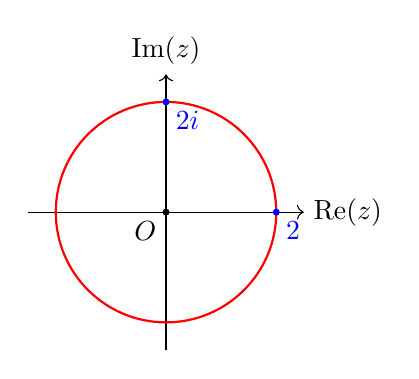
\begin{tikzpicture}[scale=0.7]
			\draw[->] (-2.5,0) -- (2.5,0) node[right] {$\Re(z)$};
			\draw[->] (0,-2.5) -- (0,2.5) node[above] {$\Im(z)$};
			\draw[thick,red] (2,0) arc (0:360:2);
			\filldraw[black] (0,0) circle (1.5pt) node[anchor=north east] {$O$};
			\filldraw[blue] (2,0) circle (1.5pt) node[anchor=north west] {$2$};
			\filldraw[blue] (0,2) circle (1.5pt) node[anchor=north west] {$2i$};
			\end{tikzpicture}
		\end{figure}
		\begin{itemize}
			\item[(a)] $\displaystyle\int_C\frac{e^z}{z}dz$\quad(b) $\displaystyle\int_C\frac{z^2}{z-1}dz$\quad(c) $\displaystyle\int_C\frac{z}{z-3}dz$\quad(d) $\displaystyle\int_C\frac{\cos z}{z\of{z^2+9}}dz$
		\end{itemize}
		\begin{proof}[\sol]
			\begin{itemize}
				\item[(a)] Let $f\of{z}=e^z$ then \[
				\oint_C\frac{e^z}{z}dz=\oint_C\frac{f\of{z}}{z-0}dz=2\pi i\cdot e^0 =2\pi i.
				\] by the Cauchy integral formula.
				\vspace{4pt}
				\item[(b)] Let $f\of{z}=z^2$ then \[
				\oint_C\frac{z^2}{z-1}dz=\oint_C\frac{f\of{z}}{z-1}dz=2\pi i\cdot(1)^2=2\pi i.
				\] by the Cauchy integral formula.
				\vspace{4pt}
				\item[(c)] Since $z_0=3$ is not inside the curve $C$, \[
				\oint_C\frac{z}{z-3}dz=0
				\] by Cauchy-Goursat theorem.
				\vspace{4pt}
				\item[(d)] Let $f\of{z}=\displaystyle\frac{\cos z}{\of{z+3i}\of{z-3i}}$ then \[
				\oint_C\frac{\of{\cos z}}{z\of{z^2+9}}dz = 2\pi i\cdot \frac{\cos 0}{3i\cdot(-3i)}=\frac{2\pi i}{9}.
				\]
			\end{itemize}
		\end{proof}
		\item 
		\begin{proof}[\sol]
			Let $f\of{\zeta}=2\zeta^2-\zeta-2$. Since $z=2$ is inside the curve $C$, \[
			g\of{2}=\oint_C\frac{2\zeta^2-\zeta-2}{\zeta-2}=2\pi i\cdot f\of{2}=2\pi i\cdot(2\cdot 2^2-2-2)=8\pi i
			\] by the Cauchy integral formula.
		\end{proof}
		\item Find the following integral. \begin{itemize}
			\item[(a)] $\displaystyle\int_0^{2\pi}e^{e^{i\theta}}d\theta$.
			\item[(b)] $\displaystyle\int_0^{2\pi}e^{-i\theta}e^{e^{i\theta}}d\theta$.
		\end{itemize}
		\begin{proof}[\sol]
			Recall that Cauchy integral formula for a function $f\of{z}$ that is analytic inside and on a simple closed contour $C$: \[
			f\of{z_0}=\frac{1}{2\pi i}\oint_C\frac{f\of{z}}{z-z_0}dz.
			\]
			\vspace{4pt}
			\begin{itemize}
				\item[(a)] Let $z = e^{i\theta}$ and $dz = ie^{i\theta} d\theta$ (\ie, $d\theta=\frac{1}{ie^{i\theta}}dz$). Then, the integral becomes: \begin{align*}
				\int_0^{2\pi}e^{e^{i\theta}}d\theta&=\oint_{\abs{z}=1}e^z\cdot\frac{1}{iz}dz\\
				&=\frac{1}{i}\oint_{\abs{z}=1}\frac{e^z}{z-0}dz\\
				&=\frac{1}{i}\cdot 2\pi i\cdot e^0\quad\text{by the Cauchy integral formula}\\
				&=2\pi.
				\end{align*}\[
				\]
				\item[(b)] Let $z = e^{i\theta}$ and $dz = ie^{i\theta} d\theta$ (\ie, $d\theta=\frac{1}{ie^{i\theta}}dz$). Then, the integral becomes: \begin{align*}
				\int_0^{2\pi}e^{-i\theta}e^{e^{i\theta}}d\theta&=\oint_{\abs{z}=1}z^{-1}\cdot e^z\cdot\frac{1}{iz}dz\\
				&=\frac{1}{i}\oint_{\abs{z}=1}\frac{e^z}{z^2}dz\\
				&=\frac{1}{i}\oint_{\abs{z}=1}\frac{e^z}{\of{z-0}^2}dz\\
				&=\frac{1}{i}\cdot 2\pi i\cdot e^0\quad\because f^{\of{1}}\of{a}=\frac{1!}{2\pi i}\oint_C\frac{f\of{z}}{\of{z-a}^{1+1}}dz\\
				&=2\pi.
				\end{align*}
			\end{itemize}
		\end{proof}
		\item 
		\begin{proof}[\sol]
			Let $f\of{\zeta}=\zeta^3+2\zeta$ then \[
			f'\of{\zeta}=3\zeta^2+2,\quad f''\of{\zeta}=6\zeta.
			\] Note that $\displaystyle f^{\of{n}}\of{z}=\frac{n!}{2\pi i}\oint_C\frac{f\of{\zeta}}{\of{\zeta-z}^{n+1}}d\zeta$. Then we have \[
			g\of{z}=\frac{2\pi i}{2!}\cdot f''\of{\zeta}=\pi i\cdot\of{6\zeta}.
			\] Thus \begin{itemize}
				\item[(i)] ($z$ is in interior of $C$) By the generalized Cauchy integral formula, \[
				g\of{z}=\pi i\cdot 6z = 6\pi iz.
				\]
				\item[(ii)] ($z$ is in exterior of $C$) By the Cauchy-Goursat theorem, \[
				g\of{z} = 0.
				\]
			\end{itemize}
		\end{proof}
		\item 
		\begin{proof}[\sol]
			Note that
			\[
			\left|\int_C f(z) dz\right| \leq ML,
			\] where $M=\max_{t\in[a,b]}\abs{f\of{\gamma\of{t}}}$ and $L = $ length of $C$.
			For $z(t) = 2e^{it}$ with $t \in [0, \frac{\pi}{2}]$, we obtain the length of the contour $C$:
			\[
			L = \int_0^{\frac{\pi}{2}} |z'(t)| dt = \int_0^{\frac{\pi}{2}} 2 dt = \pi.
			\]
			Let $\displaystyle
			f(z) = \frac{z + 4}{z^3 - 1}$ then $\displaystyle
			f(2e^{it}) = \frac{2e^{it} + 4}{(2e^{it})^3 - 1}$.
			Since
			
			\begin{align*}
			\left|f(2e^{it})\right| &= \left|\frac{2e^{it} + 4}{(2e^{it})^3 - 1}\right| \\
			&= \frac{|2e^{it} + 4|}{|8e^{3it} - 1|} \\
			&\leq \frac{2 + 4}{|8e^{3it} - 1|}.
			\end{align*}
			
			Since $|8e^{3it} - 1|$ is minimized when $t = 0$, we have:
			
			\begin{align*}
			M &= \max_{t \in [0, \frac{\pi}{2}]} \frac{6}{|8e^{3it} - 1|} \\
			&= \frac{6}{|8 - 1|} \\
			&= \frac{6}{7}.
			\end{align*}
			
			Applying the ML-inequality, we get:
			
			\[
			\left|\int_C \frac{z + 4}{z^3 - 1} dz\right| \leq ML = \frac{6}{7} \cdot \pi = \frac{6\pi}{7}.
			\]
			
			Therefore, we have proven that $\left|\int_C \frac{z + 4}{z^3 - 1} dz\right| \leq \frac{6\pi}{7}$.
			
		\end{proof}
	\end{enumerate}
	
	\footer{Department of Information Security, Cryptography and Mathematics, Kookmin University}
\end{document}
